\chapter{Progettazione Concettuale}

\section{Diagramma Delle Classi UML}

\begin{figure}[!h]
    \centering
    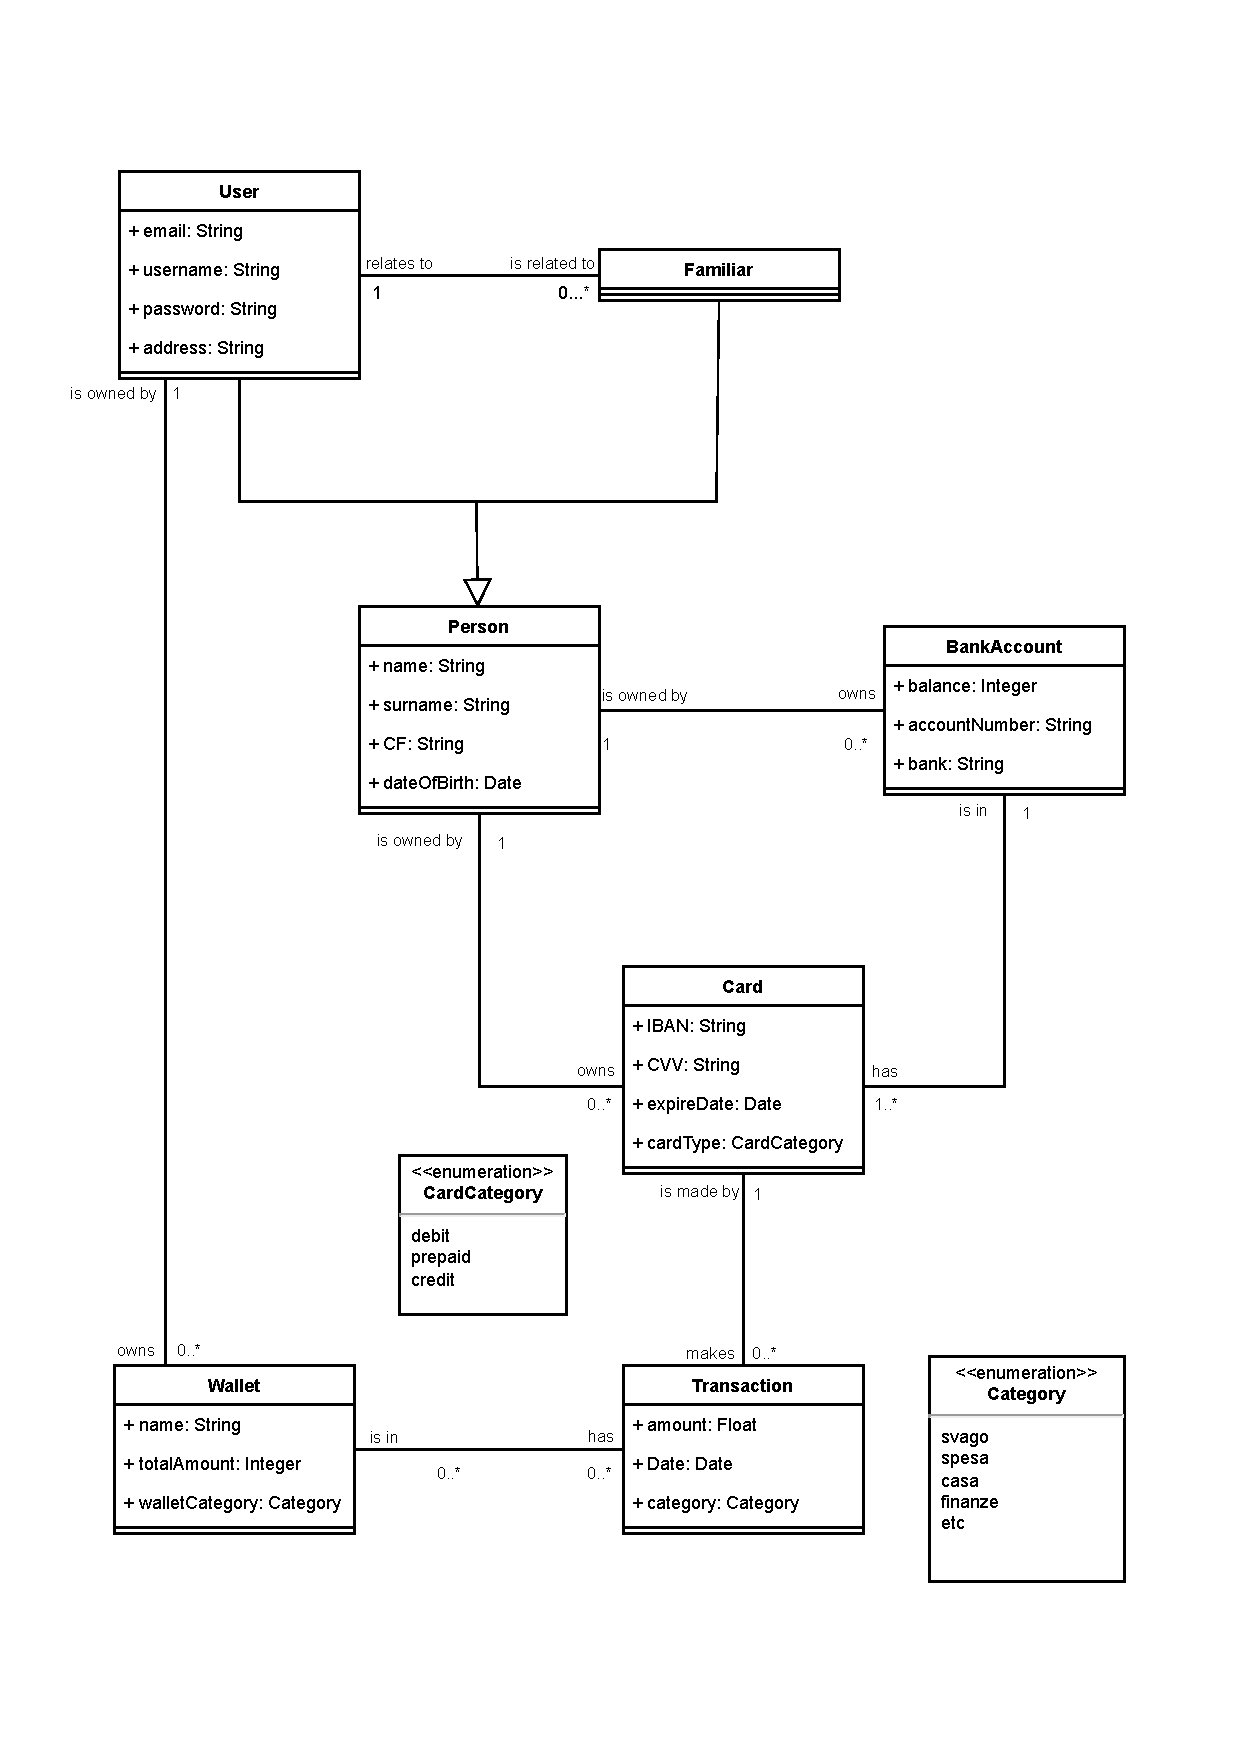
\includegraphics[scale=0.55]{pdfs/UMLdiagram.drawio.pdf}
    \caption{Diagramma UML}\label{UML}
\end{figure}

\section{Diagramma ER (Entità Relazione)}

\begin{figure}[!h]
    \centering
    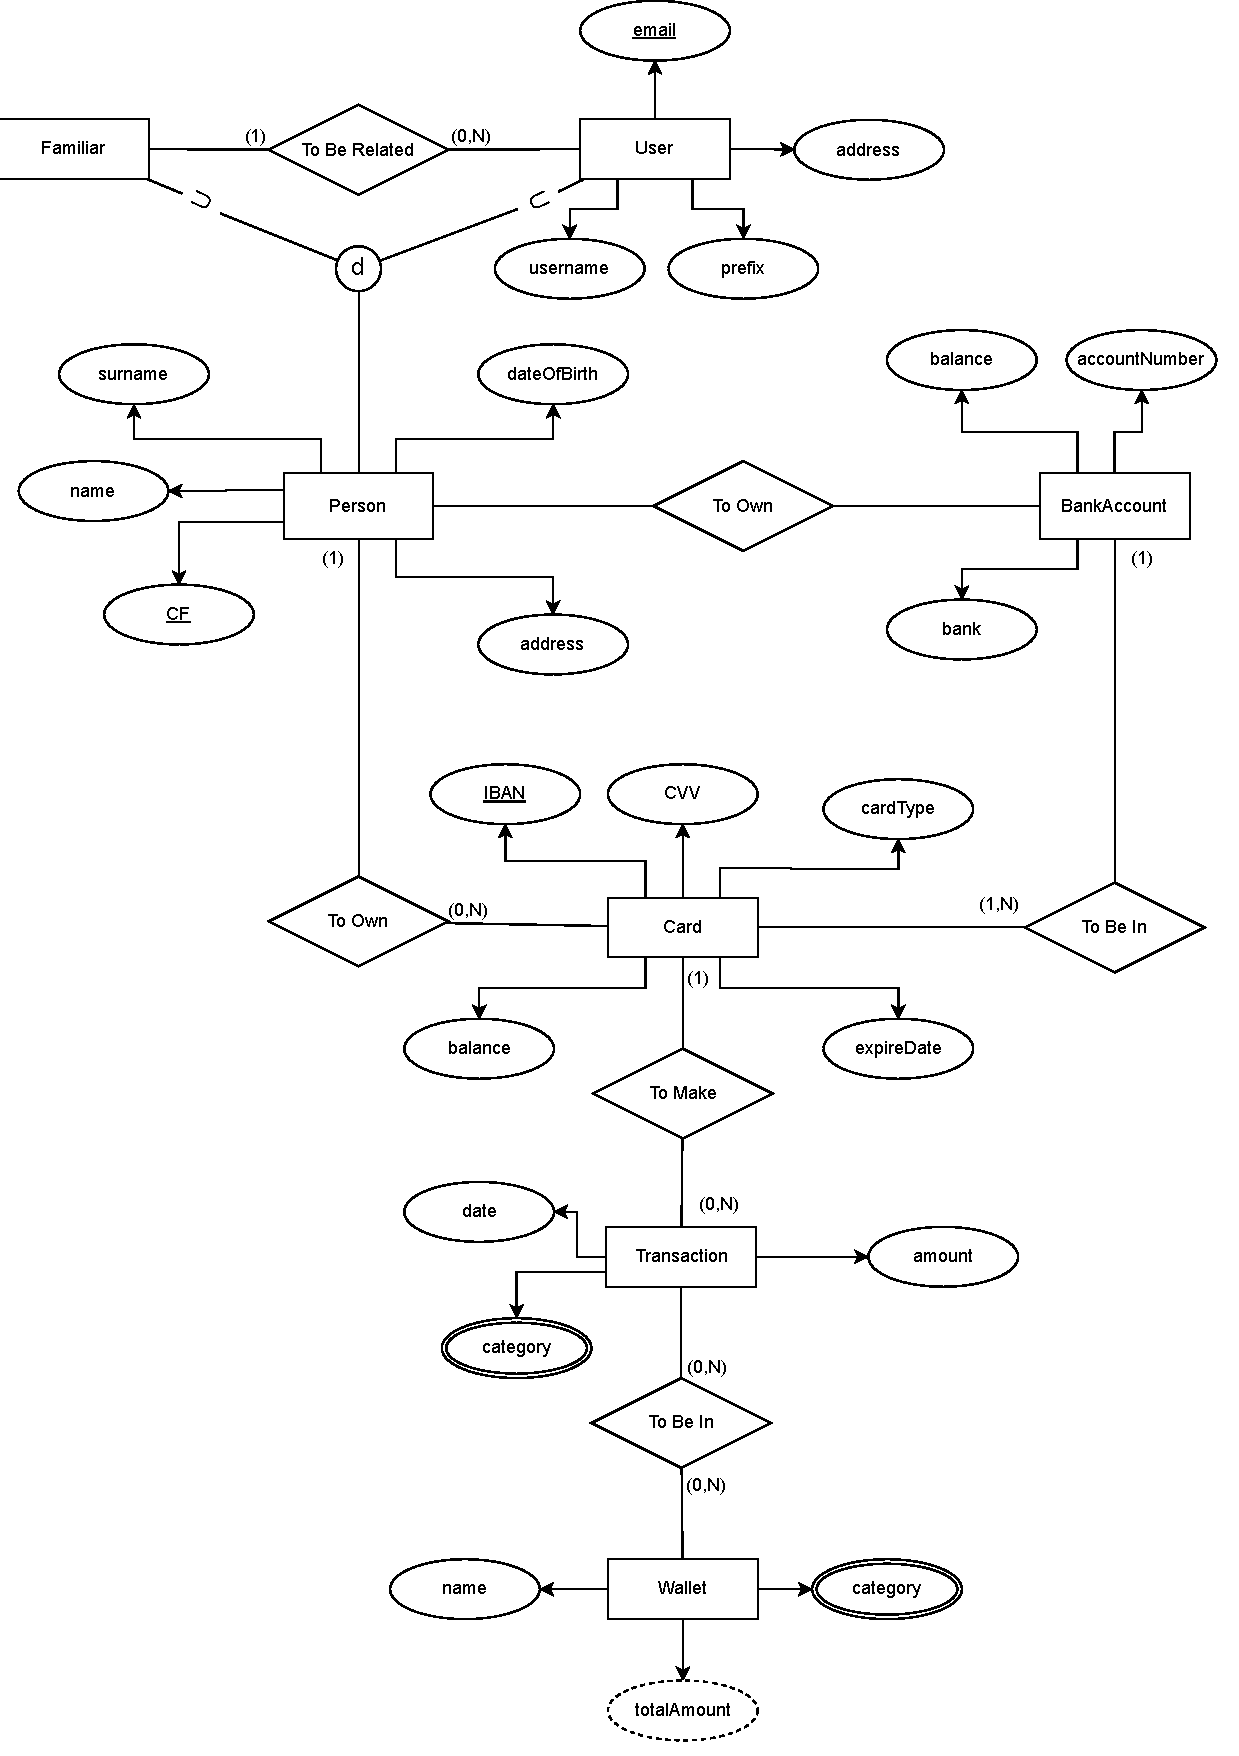
\includegraphics[scale=0.7]{pdfs/ERdiagram.drawio.pdf}
    \caption{Diagramma ER}\label{ER}
\end{figure}

\newpage

\section{Ristrutturazione}

\subsection{Attributi multipli}

Per quanto riguarda la gestione di attributi multipli,
abbiamo deciso di gestire l'attributo \textit{category} della tabella
\textbf{Transaction}, originariamente definito come enumerazione,
trasformandolo in una stringa, poiché non abbiamo bisogno di valori
specifici, trattandosi di una categoria personalizzabile.

Invece, per l'attributo \textit{cardType} della tabella \textbf{Card},
è stato deciso di non applicare lo stesso metodo, poiché le tipologie
di carte sono ben definite e non possono essere modificate.

\subsection{Generalizzazioni}

Per la generalizzazione, essendo di tipologia totale e disgiunta,
abbiamo optato per il metodo di eliminare la classe generale.
Abbiamo trasferito tutti gli attributi di essa nelle
classi specializzate, conservando le relative relazioni.

\subsection{Analisi degli identificativi}

Per la maggior parte delle classi, saranno utilizzati come identificativi
attributi già presenti di natura nelle classi stesse, poiché risultano
sufficienti e non richiedono l'uso di una chiave surrogata.
Tuttavia, in alcune classi, sono presenti chiavi surrogate,
identificate con il prefisso \textbf{ID\_}.

\newpage
\subsection{Diagramma UML ristrutturato}

\begin{figure}[!h]
    \centering
    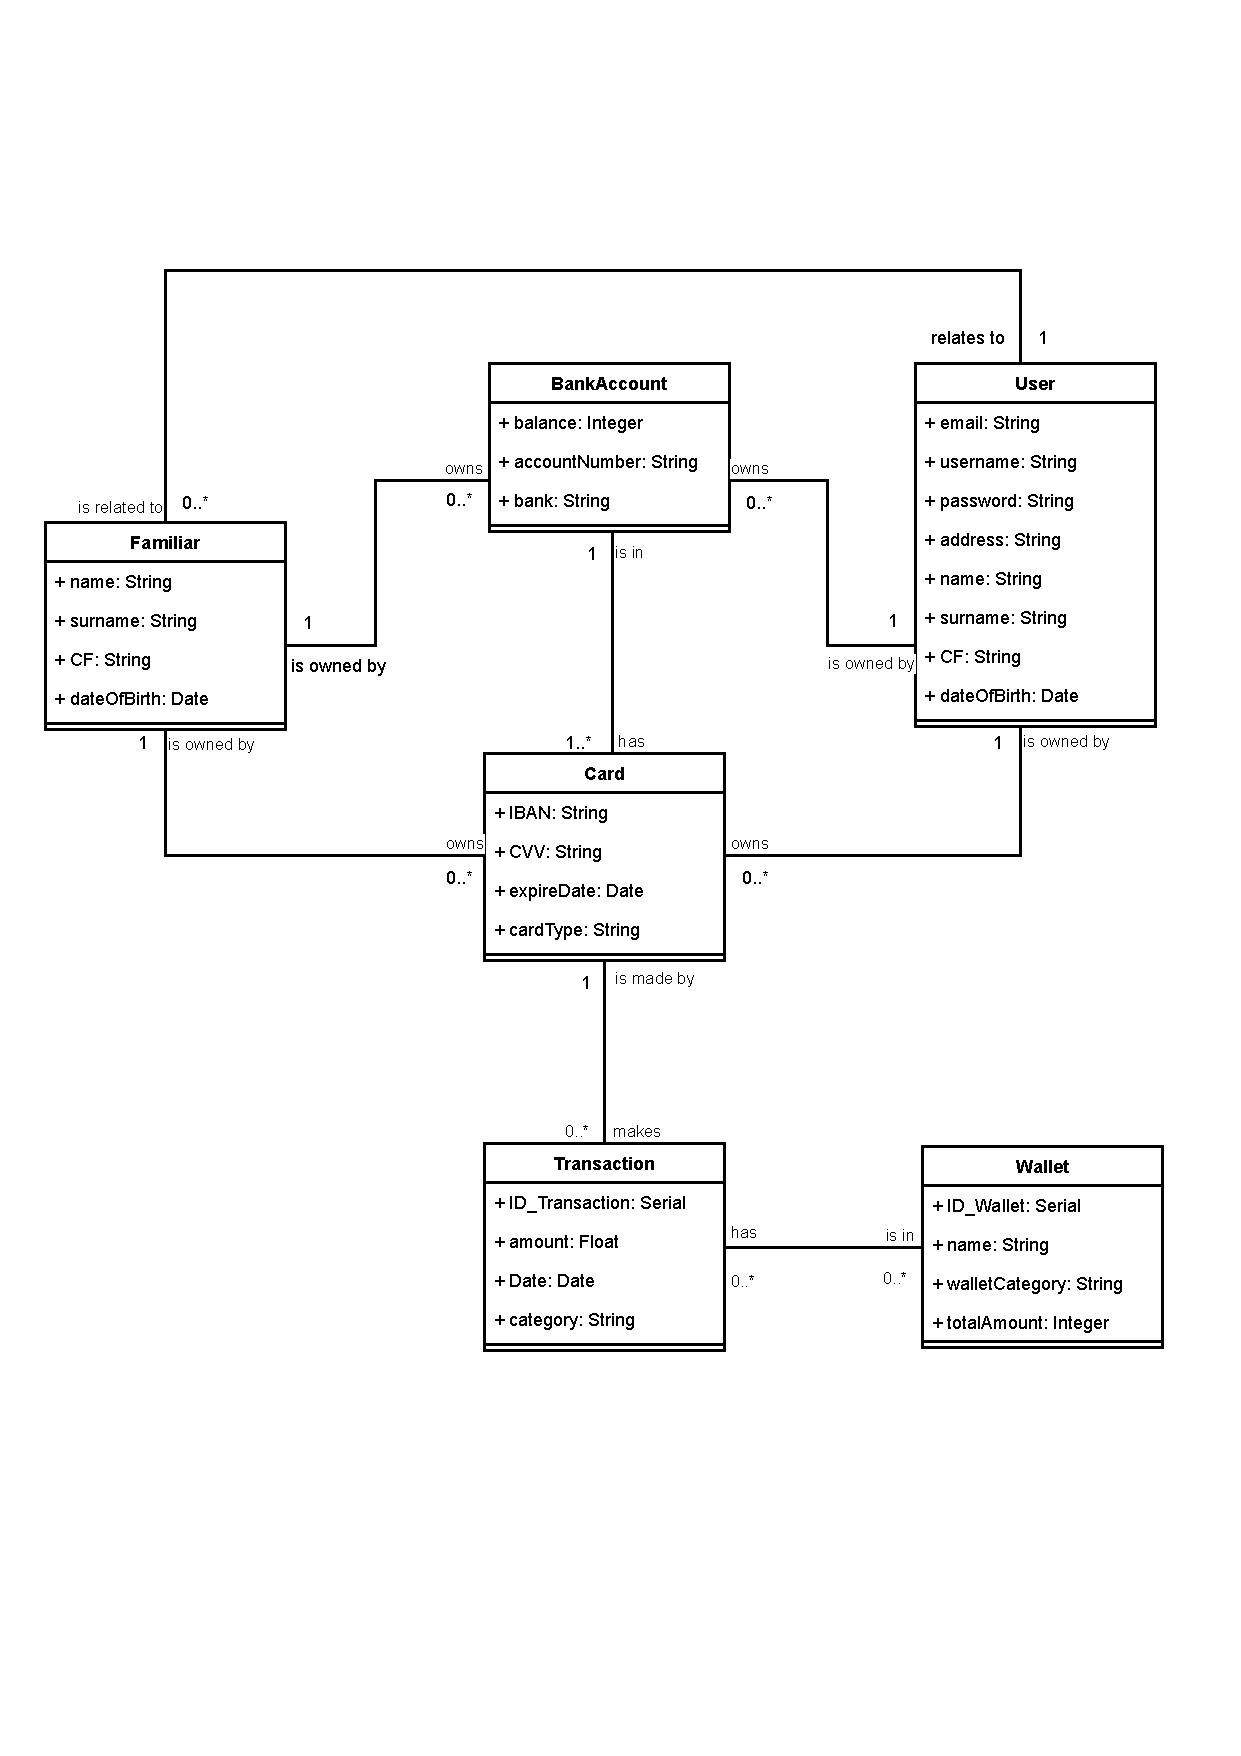
\includegraphics[scale=0.7]{pdfs/RestructuredUMLdiagram.drawio.pdf}
    \caption{Diagramma UML Ristrutturato}\label{ResUML}
\end{figure}

\newpage
\section{Dizionari}

\subsection{Dizionario delle classi}

\begin{table}[!h]

    \centering

    %13.7cm
    \begin{tabular}{m{2cm}|m{4cm}|m{7.7cm}}

         \rowcolor{black!10}Classe & Descrizione & Attributi\\ \hline

         User & Classe utilizzata per identificare gli effettivi utenti che sono registrati alla piattaforma &
         \parbox{7.7cm}{\textbf{email} (\textit{String}): email con la quale l'utente si è registrato \\ 
         \textbf{username} (\textit{String}): chiave primaria, identificativa dell'utente. È anche il nome che viene mostrato per riconoscere lo stesso \\
         \textbf{password} (\textit{String}): stringa atta alla convalidazione durante l'accesso all'account \\
         \textbf{address} (\textit{String}): indirizzo del domicilio \\
         \textbf{name} (\textit{String}): nome \\
         \textbf{surname} (\textit{String}): cognome \\
         \textbf{CF} (\textit{String}): codice fiscale \\
         \textbf{dateOfBirth} (\textit{Date}): data di nascita} \\ \hline

         Familiar & Classe utilizzata per identificare i familiari, degli utenti, che sono presenti sul database &
         \parbox{7.7cm}{\textbf{name} (\textit{String}): nome \\
         \textbf{surname} (\textit{String}): cognome \\
         \textbf{CF} (\textit{String}): codice fiscale \\
         \textbf{dateOfBirth} (\textit{Date}): data di nascita} \\ \hline
    
        \end{tabular}

\end{table}

\subsection{Dizionario delle associazioni}

\subsection{Dizionario dei vincoli}